%---------------------------------------------------------------
\chapter{Implementace mobilní aplikace}
%---------------------------------------------------------------

\begin{chapterabstract}
    V této kapitole popíšu průběh implementace mobilní aplikace, jednotlivé třídy a zajímavosti, se kterými jsem se při implementaci setkal.
\end{chapterabstract}

\section{Architektura}

Pro svou aplikaci jsem zvolil architekturu MVVM (Model View ViewModel). Aplikace se skládá ze tří vrstev -- datové, která obsahuje balíčky DTO s definicemi tříd z API, Service s třídami, které komunikují s API, business vrstvu, která obsahuje Modely s definicemi tříd, se kterými pracuje prezentační vrstva, ViewModely řešící veškerou logiku aplikace a prezentační vrstvu, která obsahuje View -- definici jednotlivých obrazovek aplikace a speciální třídu \texttt{AppState}, která zajišťuje kompatibilitu View používaných pro operační systém iOS a macOS.

\subsection{DTO}

Balíček DTO je ekvivalentem balíčku DTO na serveru. Tento balíček obsahuje definici dat, která aplikace získá z REST API. Ačkoliv jsou atributy DTO tříd na serveru a v mobilní aplikaci stejné, třídy nelze sdílet, jelikož jsou napsány v odlišných programovacích jazycích (Kotlin, Swift). Podobně jako na serveru, i v aplikaci má DTO různé typy -- základní \texttt{DTO} slouží k získávání informací z API, \texttt{EditDTO} slouží k vytváření a úpravě, \texttt{RawDTO} je zjednodušená verze základního DTO k zamezení cyklických závislostí a \texttt{SaveDTO} je určeno k uložení dat do cache v zařízení. Jednotlivá DTO implementují protokoly \texttt{Codable} \cite{swift-codable} (podporuje zakódování i dekódování), \texttt{Decodable} (podporuje pouze dekódování) nebo \texttt{Encodable} (podporuje pouze zakódování).

\begin{listing}[H]
\begin{minted}[breaklines,breaksymbolleft=]{swift}
struct SongBookDTO: Decodable {
    let id: Int
    let name: String
    let band: BandDTO
    let songs: [SongDTO]
}
struct SongBookEditDTO: Encodable {
    let name: String
    let bandId: Int
}
\end{minted}
\caption[Ukázka DTO zpěvníku v aplikaci]{Ukázka \texttt{SongBookDTO} ke čtení a \texttt{SongBookEditDTO} k úpravě}
\end{listing}

\subsection{Service}

Třídy z balíčku Service komunikují s API rozhraním za pomocí DTO a získaná data zpřístupňují ViewModelům. Jelikož je komunikace s API operace, při které probíhá přenos dat po síti, musí být metody, ve kterých probíhá komunikace s API asynchronní, aby během volání API metod nedošlo k zaseknutí uživatelského rozhraní.

Swift umožňuje volání asynchronních metod dvěma způsoby. Starší z nich využívá takzvaný \textit{completion handler}, což je funkce vyššího řádu, která je předána volající metodě jako parametr. Tato funkce se po provedení požadavku zavolá s datovým typem indikujícím úspěch, nebo chybu. Nový způsob \textit{Async API} umožňuje používat asynchronní funkce stejně jako synchronní s použitím klíčového slova \texttt{await}. Kód je tak přehlednější a srozumitelnější. \cite{swift-async-completion}

\begin{listing}[H]
\begin{minted}[breaklines,breaksymbolleft=]{swift}
func songBookList() async -> Result<[SongBookDTO], HttpStatusError> {
    let response = await networkService.get(url: Constants.songBookListUrl)
    switch response {
    case .success(let data):
        guard let songBooks = try? JSONDecoder().decode(
            [SongBookDTO].self, from: data
        ) else {
            return .failure(.badtext(
                text: "songbook_list_response_parse_error"
            ))
        }
        return .success(songBooks)
    case .failure(let error):
        return .failure(error)
    }
}
\end{minted}
\caption[Ukázka Service pro zpěvníky v aplikaci]{Ukázka metody \texttt{songBookList}, která na API odešle požadavek na získání seznamu zpěvníků. V případě úspěšného provedení požadavku se z odpovědi pokusí načíst pole DTO zpěvníků, v~případě neúspěchu pak vrátí příslušnou chybu}
\end{listing}

\subsection{Model}

Balíček Model obsahuje definici jednotlivých entit, se kterými se pracuje v aplikaci. Pro převod mezi entitami a příslušnými DTO (ať už základními, pro úpravu nebo uložení do cache) jsou použity \textit{extension properties} \cite{swift-extensions}, které umožňují přidat nové atributy do libovolné třídy bez nutnosti její úpravy. Balíček DTO jakožto součást datové vrstvy tak neobsahuje metody pro převod na jednotlivé Modely, čímž je zachována třívrstvá architektura.

\begin{listing}[H]
\begin{minted}[breaklines,breaksymbolleft=]{swift}
struct SongBook: Equatable {
    let id: Int
    let name: String
    let band: Band
    let songs: [Song]
}
\end{minted}
\caption{Ukázka Modelu zpěvníku v aplikaci}
\end{listing}

\subsection{ViewModel}

ViewModely jsou třídy, které komunikují s příslušnými třídami z balíčku Service a drží Modely, se kterými dále pracují komponenty z balíčku View. Ve ViewModelech je obsažena veškerá logika pro zpracovávání operací včetně logiky pro vytváření, úpravu, smazání nebo zobrazování dat.

\begin{listing}[H]
\begin{minted}[breaklines,breaksymbolleft=]{swift}
final class SongBookListViewModel: ObservableObject {
    @Published var state: SongBookListLoadState = .loading
    @Published var songBooks = [SongBook]()
    @Published var songsById = [String: Song]()
    
    func loadSongBooks() {
        state = .loading
        Task { await loadSongBooks() }
    }
    
    func loadSongBooks() async {
        let songBooks = await songBookService.songBookList()
        await loadSongBooks(result: songBooks)
    }
    
    @MainActor
    private func loadSongBooks(result: Result<[SongBookDTO], HttpStatusError>) async {
        switch result {
        case .success(let songBooks):
            self.songBooks = songBooks.map { song -> song.domain }
            songsById = [:] // reset song book list
            songsById = self.songBooks.flatMap { songBook -> songBook.songs }.reduce(into: songsById) { song ->
                songBook[song.idString] = song
            }
            
            appState.songBook = self.songBooks.first(where: { songBook -> songBook.id == appState.songBook?.id })
            state = .success
        case .failure(let error):
            state = .failure(error.errorDescription)
        }
    }
}
\end{minted}
\caption[Ukázka kódu z ViewModelu pro načtení seznamu zpěvníků v aplikaci]{Ukázka kódu ze \texttt{SongBookListViewModelu}, který slouží pro načtení seznamu zpěvníků a jeho zpřístupnění komponentě \texttt{SongBookListView}, která je zobrazí uživateli. Na začátku jsou definovány proměnné držící stav načítání, seznam zpěvníků a slovník písní podle jejich unikátního identifikátoru. Samotné načtení pak zajišťuje metoda  \texttt{loadSongBooks}, kde první varianta (bez klíčového slova \texttt{async}) zajistí spuštění druhé metody v asynchronním kontextu pomocí třídy \texttt{Task}, druhá varianta (s \texttt{async}) zajistí zavolání příslušné metody na \texttt{SongBookService} a poslední metoda (označená \texttt{@MainActor}) manipuluje s daty, na která je napojena komponenta View -- proto je zde použita anotace \texttt{@MainActor}, která zajistí spuštění metody na hlavním jádře}
\end{listing}

\subsection{View}

View je balíček, který obsahuje definici jednotlivých SwiftUI komponent, které tvoří uživatelské rozhraní. Tyto komponenty drží příslušný ViewModel a další pomocné proměnné, pomocí kterých je deklarativně určena aktuální podoba rozhraní.

\begin{listing}[H]
\begin{minted}[breaklines,breaksymbolleft=]{swift}
struct SongBookListView: View {
    @ObservedObject var songBookListViewModel: SongBookListViewModel

    var body: some View {
        VStack {
            switch songBookListViewModel.state {
            case .loading:
                ProgressView()
            case .failure(let error):
                ErrorView(error: error, action: songBookListViewModel.loadSongBooks, dismiss: nil)
            case .success:
                SongBookListWrapperView(songBookListViewModel: songBookListViewModel)
            }
        }
    }
}
\end{minted}
\caption[Ukázka komponenty pro zobrazení seznamu písní v aplikaci]{Ukázka komponenty \texttt{SongBookListView} pro zobrazení seznamu písní -- na základě stavu načítání z příslušného \texttt{SongBookListViewModel}u je zobrazeno buď \texttt{ProgressView} (načítací obrazovka), \texttt{ErrorView} (obrazovka zobrazující příslušnou chybovou hlášku \texttt{error} s akcemi pro znovunačtení \texttt{action} a zrušení \texttt{dismiss}), nebo obrazovka \texttt{SongBookListWrapperView} obalující seznam zpěvníků na~operačních systémech macOS a iOS.}
\end{listing}

\section{Multiplatformní aplikace}

Na základě návrhu jsem mobilní aplikaci implementoval jako nativní aplikaci pro operační systémy iOS a macOS pomocí technologie Swift. Celá aplikace je tedy rozdělena do tří částí -- \texttt{Shared}, která obsahuje sdílenou logiku a částí \texttt{macOS} a \texttt{iOS}, které každá obsahují logiku specifickou pro danou platformu.

\subsection{Uživatelské rozhraní}

Pro tvorbu uživatelského rozhraní mobilní aplikace jsem si mohl zvolit dva základní systémy tvorby rozhraní iOS / macOS aplikací. Prvním z nich jsou systémy UIKit (iOS) \cite{uikit} a AppKit (macOS) \cite{appkit}. Jedná se o specifické systémy pro tvorbu rozhraní na jednotlivé platformy. Jejich výhodou je především univerzálnost -- dá se v nich napsat bez problému jakákoliv obrazovka. Druhým je pak nový systém SwiftUI \cite{swiftui}, který je společný pro obě platformy. Není sice tak univerzální jako UIKit nebo AppKit -- při vývoji se tak může stát, že je nutné některou obrazovku napsat v těchto systémech, jeho výhodou je ale multiplatformnost -- jednou napsaný kód funguje na obou platformách.

Při tvorbě designu aplikace jsem narazil na komponenty, které nebylo možné implementovat pomocí SwiftUI. Jednalo se o seznam písní a zpěvníků, dialogy a navigační lištu.

\subsubsection{Seznam písní a zpěvníků}

Pro vytvoření seznamu prvků se ve SwiftUI používá komponenta \texttt{List} \cite{swiftui-list}. Této komponentě se předá seznam prvků a funkce, která z daného prvku vytvoří komponentu řádku seznamu. Zatímco na iOS tato komponenta obstarává posouvání seznamu, odsazení od krajů, hledání v~seznamu a rozdělení do sekcí (zpěvníků), na macOS jsou tyto funkcionality nefunkční. V seznamu na macOS navíc není funkční posouvání po prvcích pomocí šipek na klávesnici. Seznam písní a zpěvníků jsem tak musel na platformě macOS implementovat vlastním řešením s pomocí SwiftUI komponenty \texttt{LazyVStack} \cite{swiftui-lazyvstack}, která pouze vykreslí předané prvky pod sebe. Logiku posouvání seznamu, odsazení od krajů, hledání v seznamu a posouvání pomocí šipek jsem pak implementoval pomocí technologie UIKit.

\begin{figure}[H]
    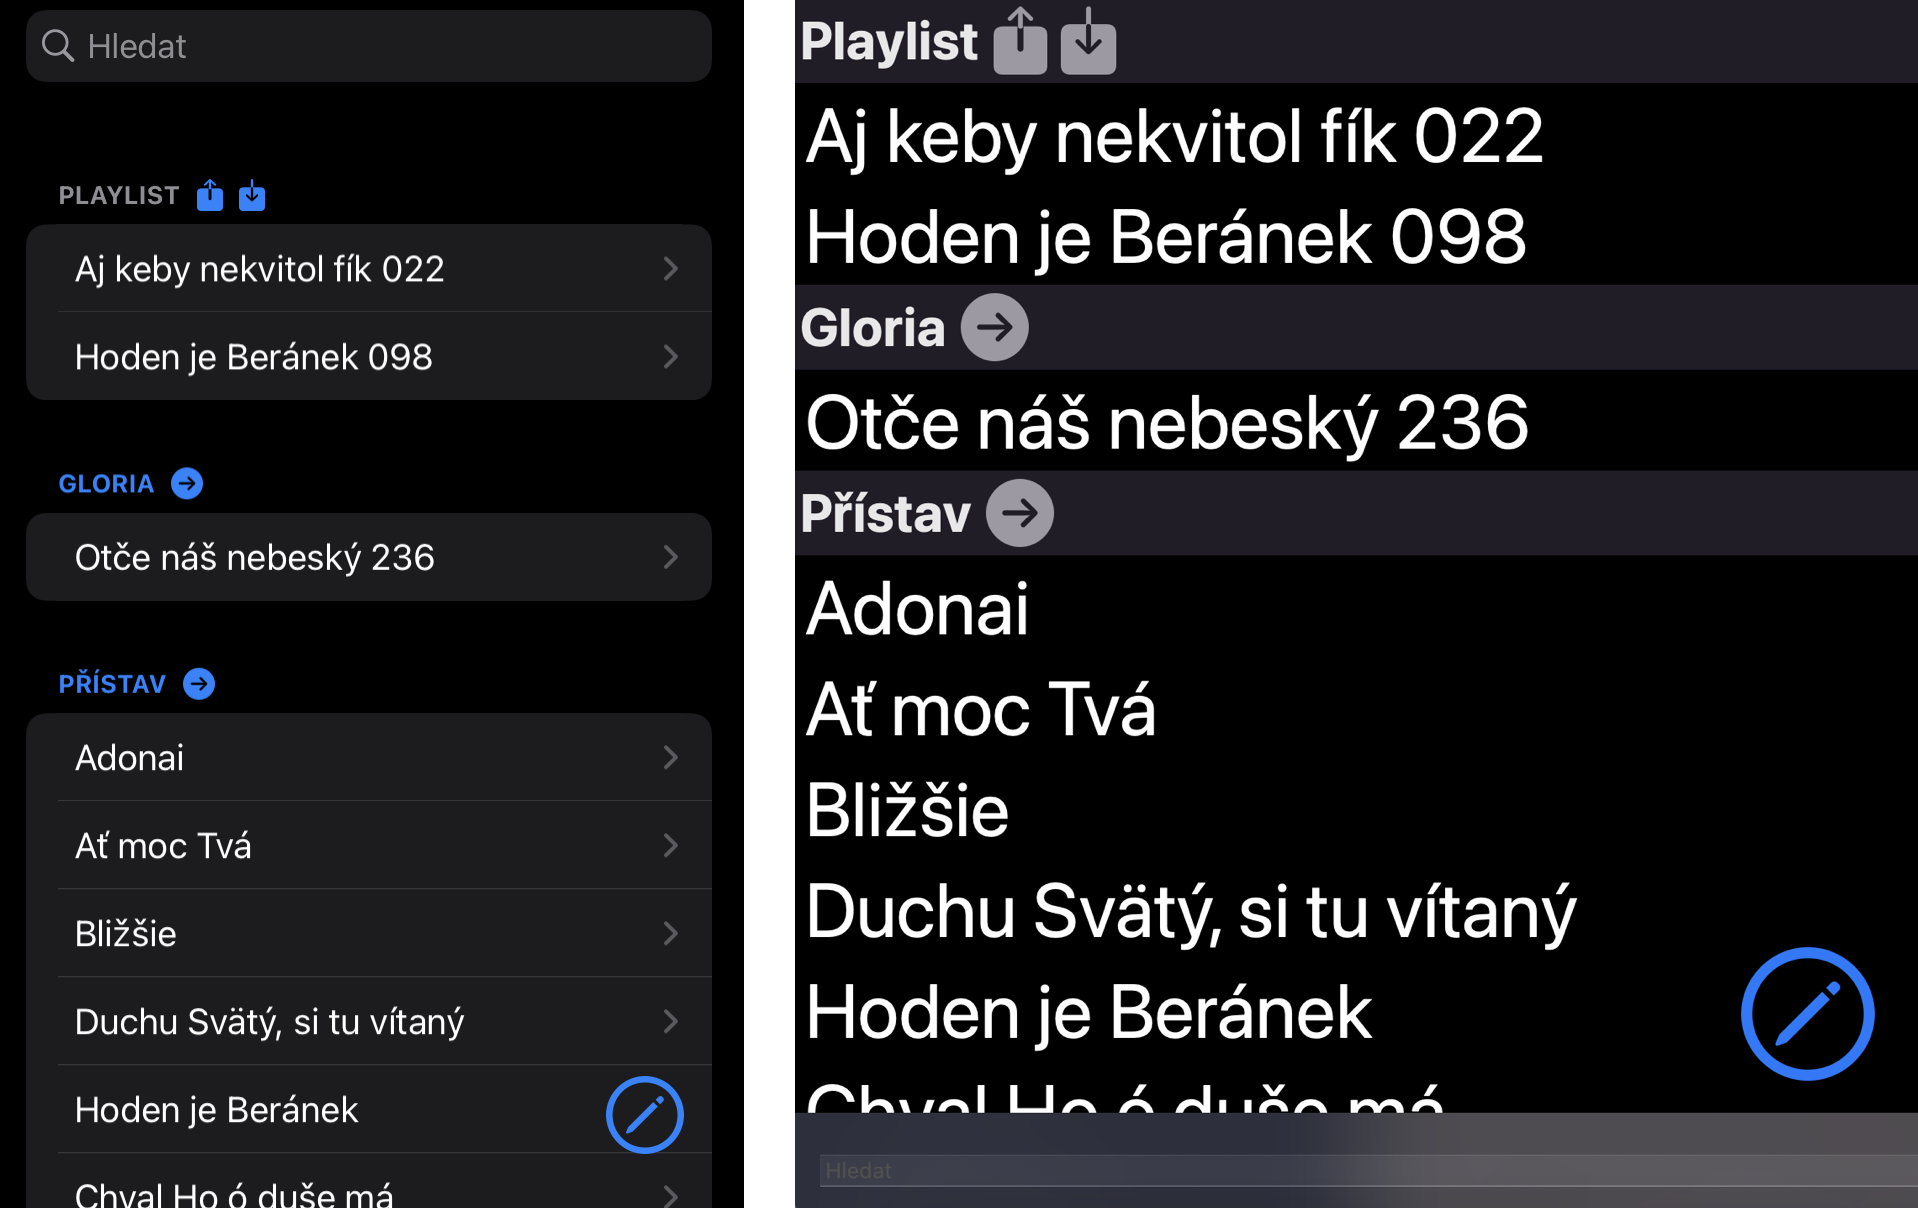
\includegraphics[width=\textwidth]{images/5-implementace/5-1-seznam-zpevniku.png}
    \caption[Seznam písní a zpěvníků -- rozdíl mezi iOS a macOS]{Seznam písní a zpěvníků -- vlevo nativní \texttt{List} řešení na systému iOS, vpravo vlastní řešení pro systém macOS s využitím SwiftUI komponenty \texttt{LazyVStack}}
\end{figure}

\subsubsection{Dialogy a navigační lišta}

Jelikož je iOS operační systém pro mobilní zařízení, zatímco macOS pro notebooky a počítače, je nativní chování prvků v navigační liště odlišné. Zatímco macOS podporuje v navigační liště tlačítka jak vlevo, tak vpravo, u iOS můžou být tlačítka přítomna pouze vpravo, jelikož se vlevo ukazuje nativní tlačítko pro návrat na předchozí obrazovku. Toto tlačítko pro návrat na předchozí obrazovku pak musí být v systému macOS tam, kde je potřeba (narozdíl od systému iOS totiž není povinné pro každou obrazovku), implementováno samostatně.

\begin{figure}[H]
    
\includegraphics[width=\textwidth]{images/5-implementace/5-2-navigacni-lista.png}
    \caption[Navigační lišta -- rozdíl mezi iOS a macOS]{Navigační lišta -- vlevo iOS s nativním tlačítkem pro návrat na obrazovku seznam zpěvníků, vpravo macOS s tlačítkem pro navigaci do nastavení. Na obou platformách je pak vpravo tlačítko pro zobrazení \texttt{popover} dialogu pro nastavení písně}
\end{figure}

Také způsob zobrazování dialogů na jednotlivých platformách je odlišný -- na macOS se typ dialogu \texttt{sheet} zobrazuje jako nové okno, nativně ale neobsahuje tlačítko pro zavření. Tlačítka se mu tak musí předat do navigační lišty s umístěním dolů. Na iOS je \texttt{sheet} dialog možné schovat potáhnutím prstu dolů, tlačítko pro odeslání je pak umístěno v navigační liště nahoře.

\begin{figure}[H]
    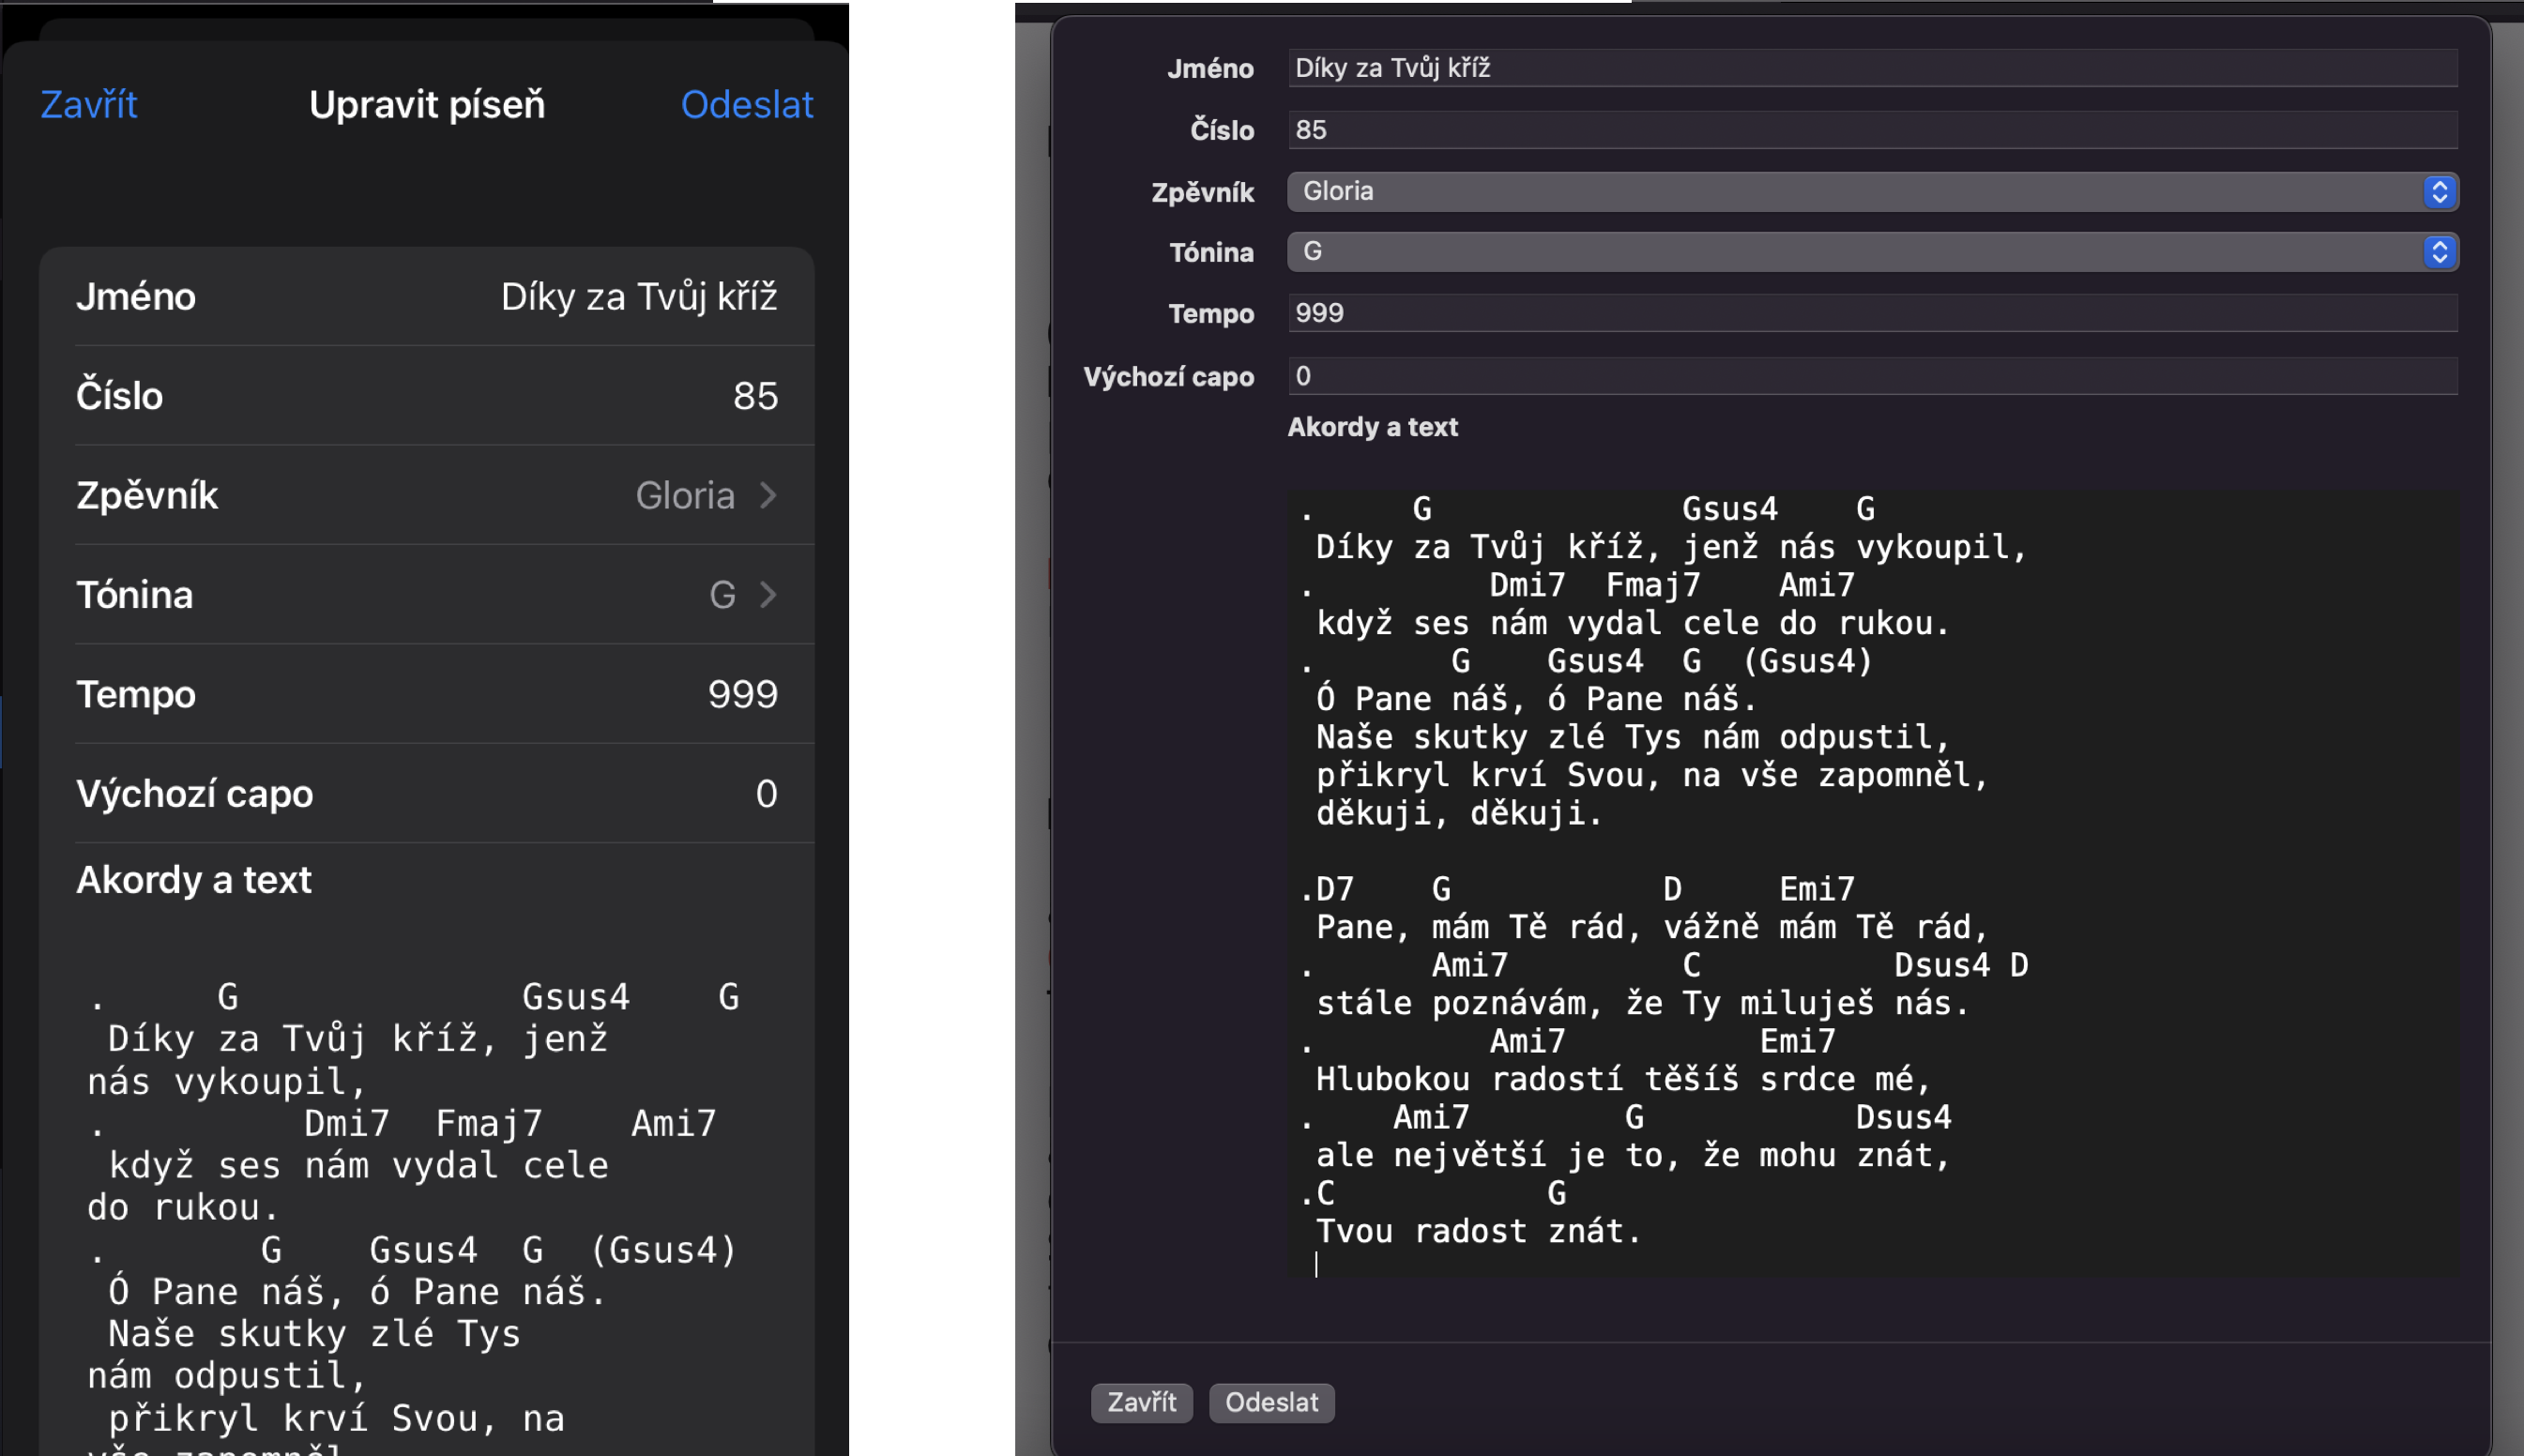
\includegraphics[width=\textwidth]{images/5-implementace/5-3-dialog-sheet.png}
    \caption[Úprava písně -- rozdíl mezi iOS a macOS]{Úprava písně -- vlevo iOS \texttt{sheet} dialog přes celou obrazovku s tlačítky nahoře a možností zavřít potáhnutím dolů, vpravo macOS \texttt{sheet} dialog jako nové okno s tlačítky dole v navigační liště}
\end{figure}

\subsection{Navigační logika}

Jak v iOS, tak v macOS aplikacích funguje navigace odlišně. V iOS aplikaci se používá způsob navigace \texttt{stack} -- uživatel vždy vidí právě jednu obrazovku, zatímco v macOS aplikaci je povinný způsob navigace \texttt{columns} -- uživatel vidí dva sloupce, kdy v levém je typicky seznam prvků a v~pravém detail prvku. Toto chování nativně zajišťuje komponenta \texttt{NavigationView} \cite{swiftui-navigationview}, které lze na základě platformy nastavit způsob navigace. Přechod mezi obrazovkami pak aplikace provádí pomocí komponenty \texttt{NavigationLink} \cite{swiftui-navigationlink}.

Při použití komponenty \texttt{NavigationView} a \texttt{NavigationLink} na systému iOS vše fungovalo správně. Když jsem ale tyto komponenty použil na systému macOS, detaily písní, které se měly zobrazovat v pravém sloupci, náhodně mizely. Pro macOS jsem tedy musel vytvořit vlastní řešení, které v rámci komponenty \texttt{NavigationView} zajišťuje přechod mezi obrazovkami bez použití komponenty \texttt{NavigationLink}.

\section{Dependency Injection}

Ve Swiftu sice existují externí frameworky řešící Dependency Injection, jejich použití je ale zbytečně příliš komplexní, proto jsem se rozhodl pro použití čistého Swift řešení \textit{protocol-oriented programming} \cite{protocol-oriented-programming}. Každá Service implementuje protokol \texttt{Servicing}, na kterém jsou závislé jednotlivé ViewModely. V celé aplikaci je pak k dispozici třída \texttt{DI}, které jsou předány jednotlivé Services pomocí \textit{extension property} a protokolu \texttt{HasServicing}.

\begin{listing}
\begin{minted}[breaklines,breaksymbolleft=]{swift}
// ContentView.swift
NavigationView {
    SongBookListView(songBookListViewModel: songBookListViewModel)
    if let song = appState.song { SongView(song: song) }
    else { Text("no_song_selected") }
}.navigationViewStyle(.columns)

// SongBookListView.swift
songListView.onTapGesture { appState.song = song }
\end{minted}
\caption[Navigační logika aplikace v systému macOS]{Navigační logika aplikace v systému macOS -- v \texttt{NavigationView} je jako první (zobrazí se vlevo) vždy komponenta pro seznam zpěvníků a pokud je ve třídě \texttt{AppState} nastavena aktuální píseň, zobrazí se její detail, jinak se zobrazí text informující uživatele o tom, že žádná píseň nebyla vybrána}
\end{listing}

\begin{listing}
\begin{minted}[breaklines,breaksymbolleft=]{swift}
// ContentView.swift
NavigationView {
    SongBookListView(songBookListViewModel: songBookListViewModel)
}.navigationViewStyle(.stack)

// SongBookListView.swift
NavigationLink(
    destination: SongView(songBook: songBook),
    tag: song.idString,
    selection: songBookViewModel.selectedSongId
) { songListView }
\end{minted}
\caption[Navigační logika aplikace v systému iOS]{Navigační logika aplikace v systému iOS -- v \texttt{NavigationView} je pouze komponenta pro seznam zpěvníků, přechod na detail písně provádí systém pomocí komponenty \texttt{NavigationLink}}
\end{listing}

\begin{listing}
\begin{minted}[breaklines,breaksymbolleft=]{swift}
// SongBookService.swift
protocol SongBookServicing {
    func songBookList() async -> Result<[SongBookDTO], HttpStatusError>
}
protocol HasSongBookService {
    var songBookService: SongBookServicing { get }
}

private let _songBookService = SongBookService(context: context)
extension DI: HasSongBookService {
    var songBookService: SongBookServicing { _songBookService }
}

// SongBookListViewModel.swift
private let songBookService: SongBookServicing
init(context: HasSongBookService) {
    songBookService = context.songBookService
}
\end{minted}
\caption[Ukázka použití protocol-oriented programming v aplikaci]{Ukázka použití protocol-oriented programming ve třídě Service pro zpěvníky, která dědí z protokolu \texttt{SongBookServicing}, na kterém závisí ViewModel pro seznam písní. Předání \texttt{SongBookService} do ViewModelu pak probíhá pomocí třídy \texttt{DI}.}
\end{listing}

\section{Dělení textu písně}

Při programování obrazovky detailu písně jsem se nečekaně setkal s problémem při zalamování textu a akordů písně. Při použití nativní SwiftUI komponenty \texttt{Text} \cite{swiftui-text} se jinak zalamovaly řádky s akordy a jinak řádky s textem. Toto zalomení způsobilo nesprávnou polohu akordů vůči jednotlivým slovům textu, což činilo aplikaci nepoužitelnou na menších zařízeních s větší velikostí textu.

\begin{figure}[H]
    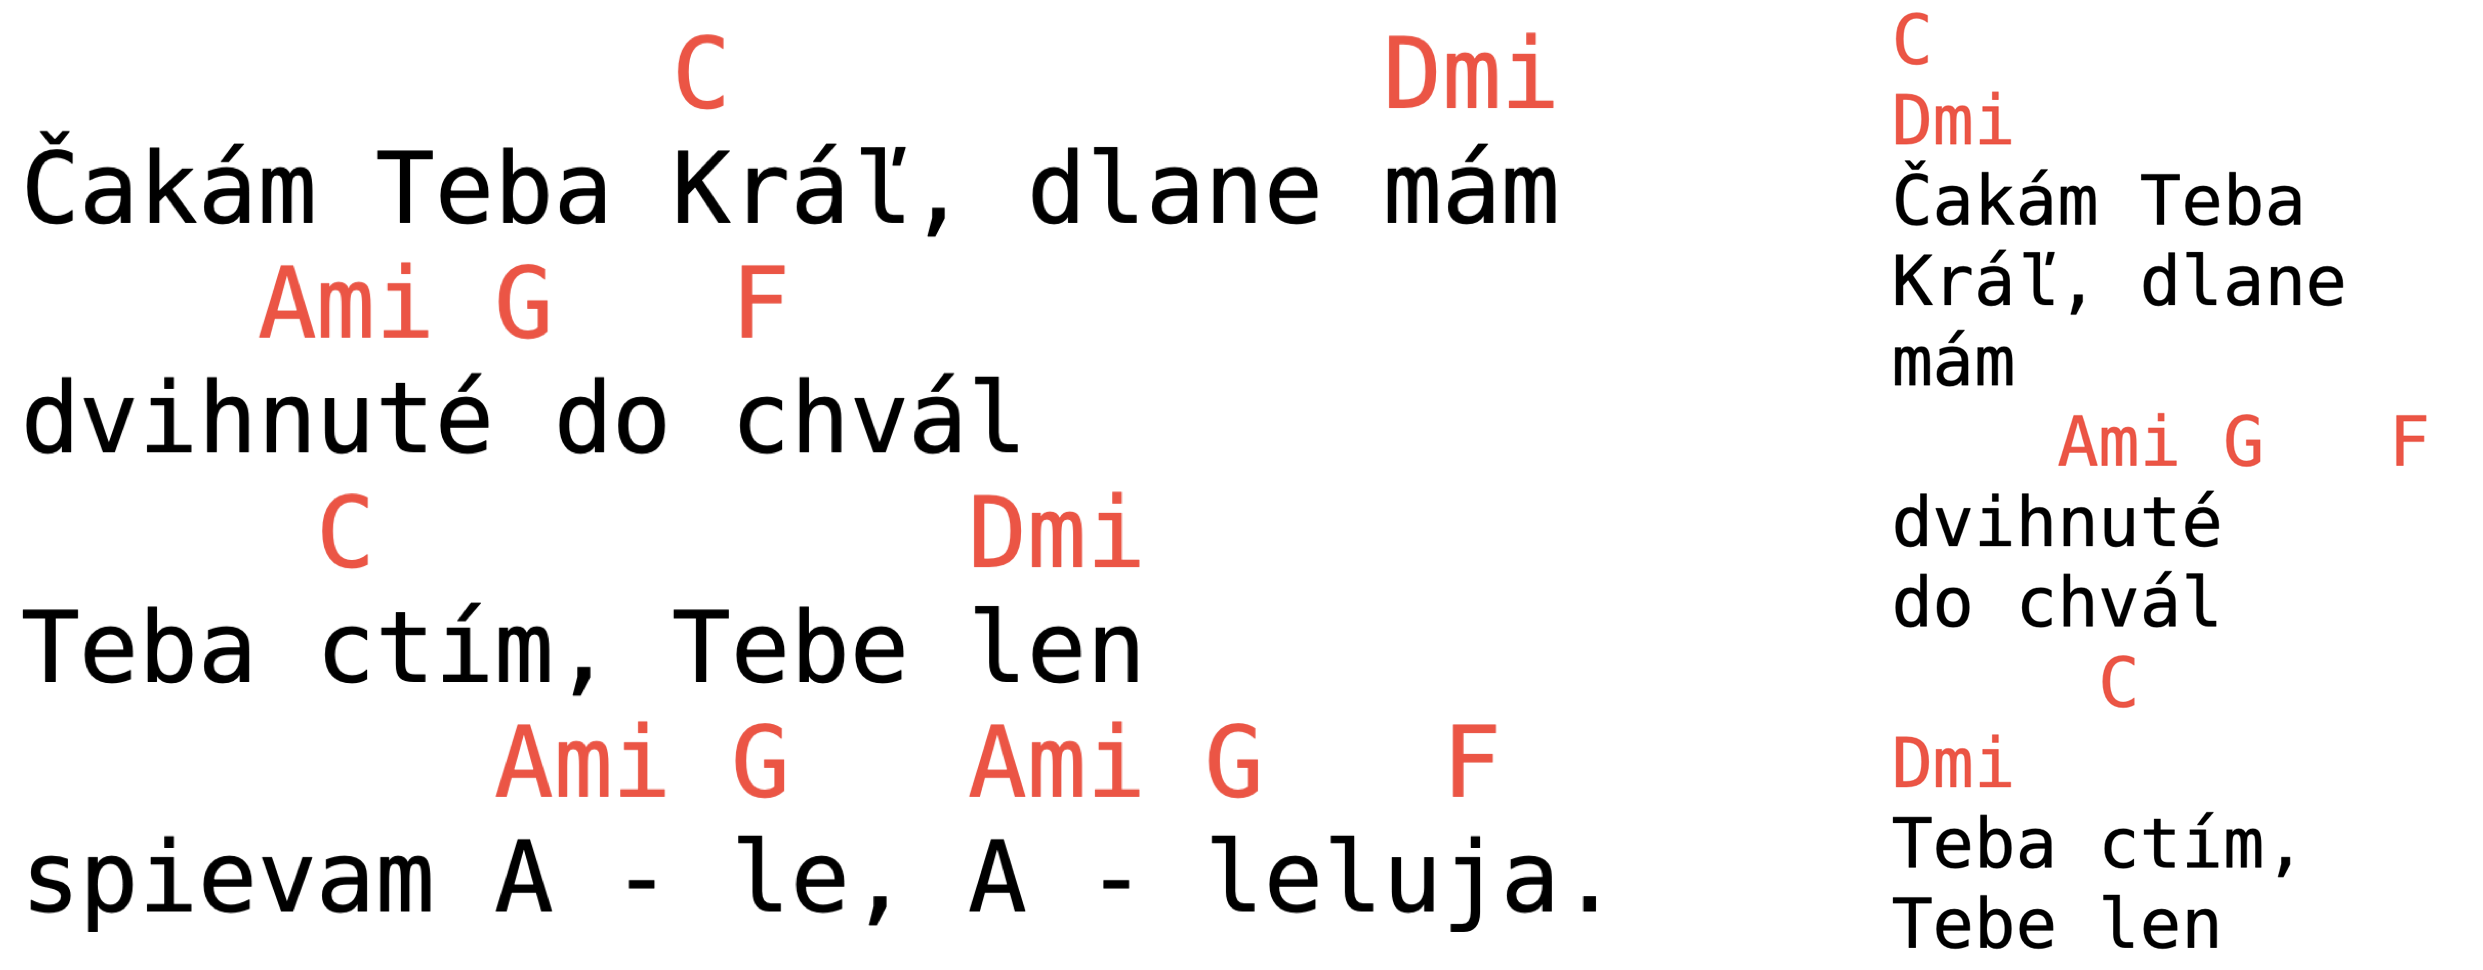
\includegraphics[width=\textwidth]{images/5-implementace/5-4-spatne-zalomeni.png}
    \caption[Ukázka nesprávného zalamování textu v detailu písně]{Ukázka nesprávného zalamování textu v detailu písně -- vlevo je původní text, vpravo nesprávně zalomený text -- akordy jsou v nesprávné poloze}
\end{figure}

Při průzkumu stávajících řešení zalamování textu jsem zjistil, že pro technologii SwiftUI aktuálně narozdíl od jiných technologií jako je CSS neexistuje nativní řešení ani jednoduše použitelná knihovna, která by umožnila text správně zalomit. Rozhodl jsem se proto implementovat vlastní algoritmus, který text rozdělí na základě maximálního možného počtu znaků, které se vejdou na obrazovku na šířku a jelikož neexistuje nativní řešení ani knihovna pro zjištění tohoto maximálního počtu znaků, implementoval jsem také jeho výpočet.

\begin{figure}[H]
    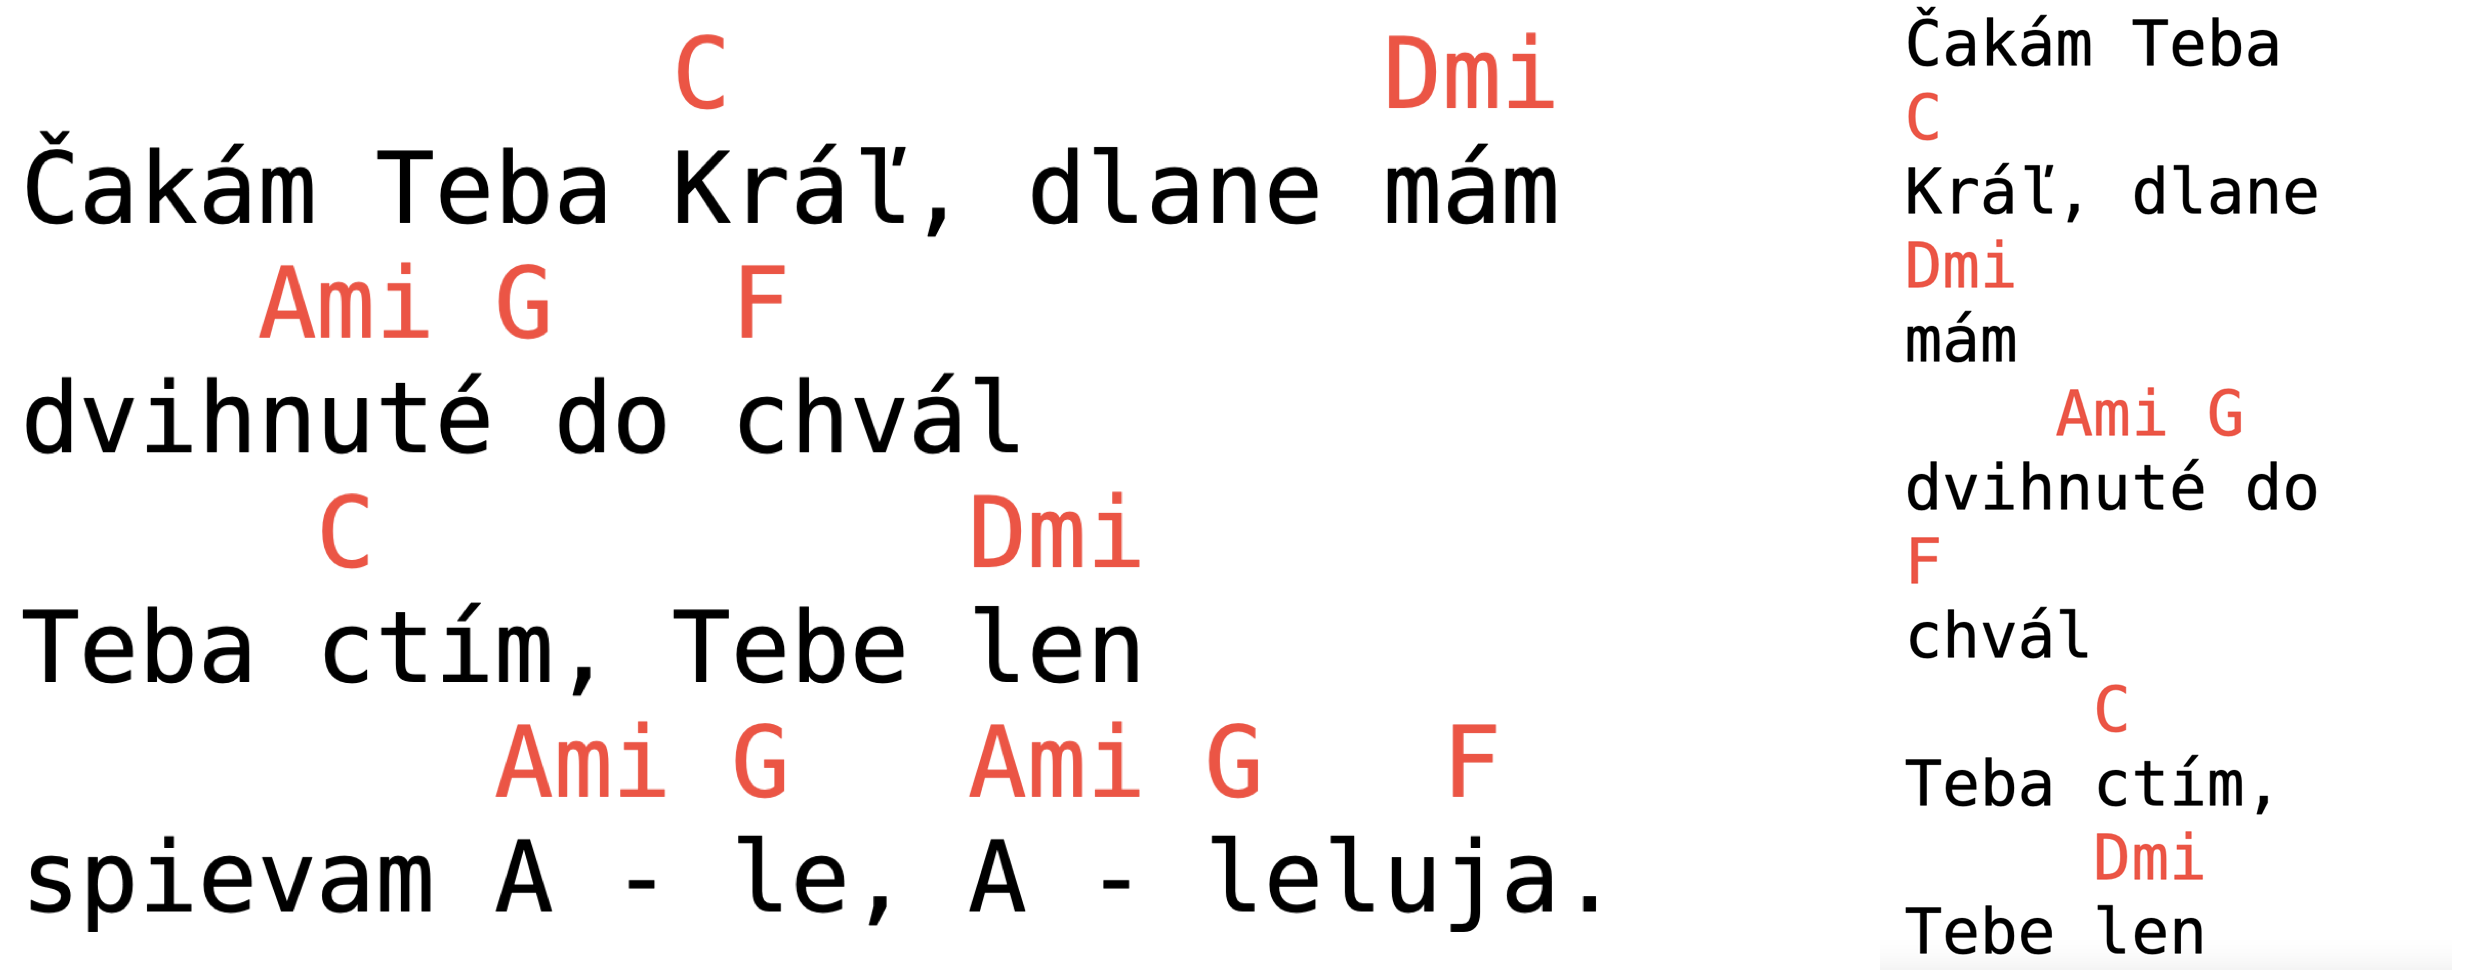
\includegraphics[width=\textwidth]{images/5-implementace/5-5-spravne-zalomeni.png}
    \caption[Ukázka správného zalamování textu v detailu písně]{Ukázka správného zalamování textu v detailu písně -- vlevo je původní text, vpravo zalomený text -- je zachována poloha všech akordů}
\end{figure}

Dělení textu tak, aby bylo na řádce maximálně N znaků pak probíhá algoritmicky nalezením poslední pozice v prvních N znacích, na které je jak v akordech, tak v textu mezera. Pokud taková pozice neexistuje, text je rozdělen po N znacích bez ohledu na mezery.

\begin{listing}
\begin{minted}[breaklines,breaksymbolleft=]{swift}
// SongWidthReaderView.swift
struct SongWidthReaderView<Content>: View where Content: View {
    @ObservedObject var songViewModel: SongViewModel
    let content: (Int) -> Content
    
    var body: some View {
        ZStack {
            ScrollView {
                VStack {
                    if let maxChars = songViewModel.maxLineChars {
                        HStack {
                            content(maxChars)
                            Spacer()
                        }
                    }
                    
                    Text("X")
                        .hidden()
                        .font(.custom(
                            "Bitstream Vera Sans Mono",
                            size: songViewModel.textSize
                        ).monospaced())
                        .readWidth(songViewModel.textWidth)
                }
            }
        }
        .readWidth(songViewModel.viewWidth)
    }
}

// SongViewModel.swift
@Published var maxLineChars: Int? = nil

@Published var textWidth: Double? = nil {
    didSet { calculateMaxLineChars() }
}

@Published var viewWidth: Double? = nil {
    didSet { calculateMaxLineChars() }
}

private func calculateMaxLineChars() {
    guard let textWidth = textWidth, let viewWidth = viewWidth else { return }
    maxLineChars = Int(viewWidth / textWidth)
}
\end{minted}
\caption[Ukázka pomocné třídy pro zalamování textu v aplikaci]{Třída \texttt{SongWidthReaderView} počítá maximální počet znaků, které se vejdou na obrazovku jako šířku celé obrazovky (metoda \texttt{readWidth} na komponentě \texttt{ZStack}) dělenou šířkou jednoho znaku (metoda \texttt{readWidth} na komponentě \texttt{Text}, která je skrytá metodou \texttt{hidden}). Jakmile je přečtena šířka obrazovky i znaku, je nastaven maximální počet znaků a předán komponentě \texttt{content}, která správně rozdělí text a akordy písně a zobrazí je uživateli}
\end{listing}

\section{Transpozice}

Jednou z častých úprav akordů, kterou členové hudebního doprovodu provádí, je takzvaná \textit{transpozice akordů}. Jedná se o posun akordů z jedné tóniny do jiné o daný počet půltónů. Tento posun se provádí z různých důvodů, mezi nejčastější z nich patří usnadnění zpěvu nebo hry na nástroj. \cite{transpozice}. Problémem ale je, že každý hudebník nepoužívá stejnou transpozici -- například klavírista hraje v originální tónině, zatímco kytarista použije transpozici -3 a nasadí kapodastr na třetí pražec. V aplikaci jsem se proto rozhodl transpozici umožnit a nazval jsem ji \textit{capo} (z anglického capodastr).

\begin{figure}[H]
    \centering
    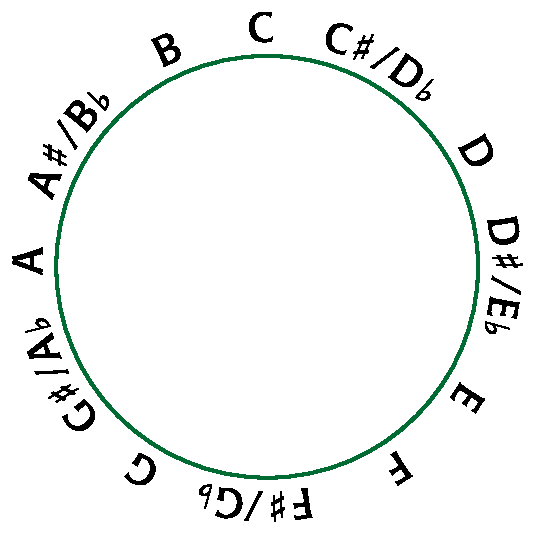
\includegraphics[width=0.6\textwidth]{images/5-implementace/5-6-chromaticky-kruh.pdf}
    \caption[Chromatický kruh znázorňující posloupnost akordů při transpozici]{Chromatický kruh znázorňující posloupnost 12 akordů při transpozici \cite{chromatic-circle}}
\end{figure}

Algoritmická transpozice akordů probíhá vytvořením pole všech 12 tónin. Pro každý akord v~textu je nalezena jeho tónina, index této tóniny v poli tónin a k tomuto indexu je přičten nebo odečten počet půltónů. Na výsledném indexu se pak nachází transponovaný akord.

\begin{listing}[H]
\begin{minted}[breaklines,breaksymbolleft=]{swift}
let transposed = original.map { chord -> (String, String) in
    for key in SongKey.allCases {
        let transposed = key.transpose(steps: capo, keys: keys)
        if chord.replacingOccurrences(of: "(", with: "").starts(with: key.localized) {
            return (chord, chord.replacingOccurrences(of: key.localized, with: transposed.localized))
        }
    }
    return (chord, chord)
}
\end{minted}
\caption{Ukázka algoritmu pro transpozici akordů}
\end{listing}

Při takovéto transpozici jsem musel řešit dva problémy. Prvním problémem je různé značení jednotlivých tónin -- například tónina C\musSharp{} dur je pro účely aplikace ekvivalentní s tóninou D\musFlat{} dur. V aplikaci jsem tedy do nastavení přidal možnost volby, zda se mají akordy transponovat podle původní tóniny písně, nebo se mají použít vždy křížky/béčka.

\begin{listing}[H]
\begin{minted}[breaklines,breaksymbolleft=]{swift}
var skip = 0
let result = transposed.compactMap { pair -> String? in
    let originalStr = pair.0, transposedStr = pair.1

    // Odstranění přebytečných mezer
    if skip > 0 && transposedStr.isEmpty {
        skip -= 1
        return nil
    }
    
    // OK, transpozice nemění počet znaků
    if originalStr.count == transposedStr.count {
        return transposedStr
    }
    
    // Počet znaků je nyní menší = přidáme mezeru
    if transposedStr.count < originalStr.count {
        return transposedStr + " "
    }
    
    // Počet znaků je větší, zvětšíme rozdíl
    skip += 1
    return transposedStr
}
\end{minted}
\caption{Ukázka algoritmu, který po transpozici opraví polohu akordů vůči textu}
\end{listing}

Druhý problém je způsoben rozdílnou délkou akordů během transpozice -- například akord C má jeden znak a C\musSharp{} má 2 znaky, což způsobuje, že se při transpozici mění poloha akordů vůči textu. Tento problém jsem vyřešil tak, že si při transpozici akordů pamatuji také původní akord a po transpozici všech akordů projdu postupně všechny akordy na řádku a pamatuji si rozdíl mezi počtem znaků transponovaných akordů a původních akordů. Kdykoliv se pak mezi akordy objeví více než jedna mezera, smažu přebytečné mezery s cílem zachování původní polohy akordů.

\section{Lokalizace}

Jedním z nefunkčních požadavků na aplikaci je podpora češtiny a polštiny. SwiftUI lokalizaci nativně podporuje -- pokud je do nativní komponenty předán textový řetězec, pokusí se ho nejprve najít v lokalizační tabulce \texttt{Localizable.strings} jazyka, který uživatel zvolil pro aplikaci, případně jazyka systému. Pokud tento řetězec v dané tabulce existuje, je přeložen, jinak je jako text použit klíč samotný. SwiftUI komponenty ale nativně nepřekládají texty, které jsou do nich vloženy v proměnných. Takové texty musí být přeloženy manuálně voláním makra \texttt{NSLocalizedString} \cite{swift-localizedstring}.
